\documentclass{article}
\usepackage{amsmath,amssymb,amsfonts,graphicx}
\usepackage{blindtext}
\usepackage{mdframed}
\usepackage{multicol}
\usepackage{wrapfig}

\title{
\textbf{Visualization and Connectedness of Quadratic Julia Sets}
}
\author{Emily Prieto}
\date{}
\pagestyle{empty}

\begin{document}

\maketitle
\vspace{-0.5in}
\begin{figure}[htb!]
	\centering
	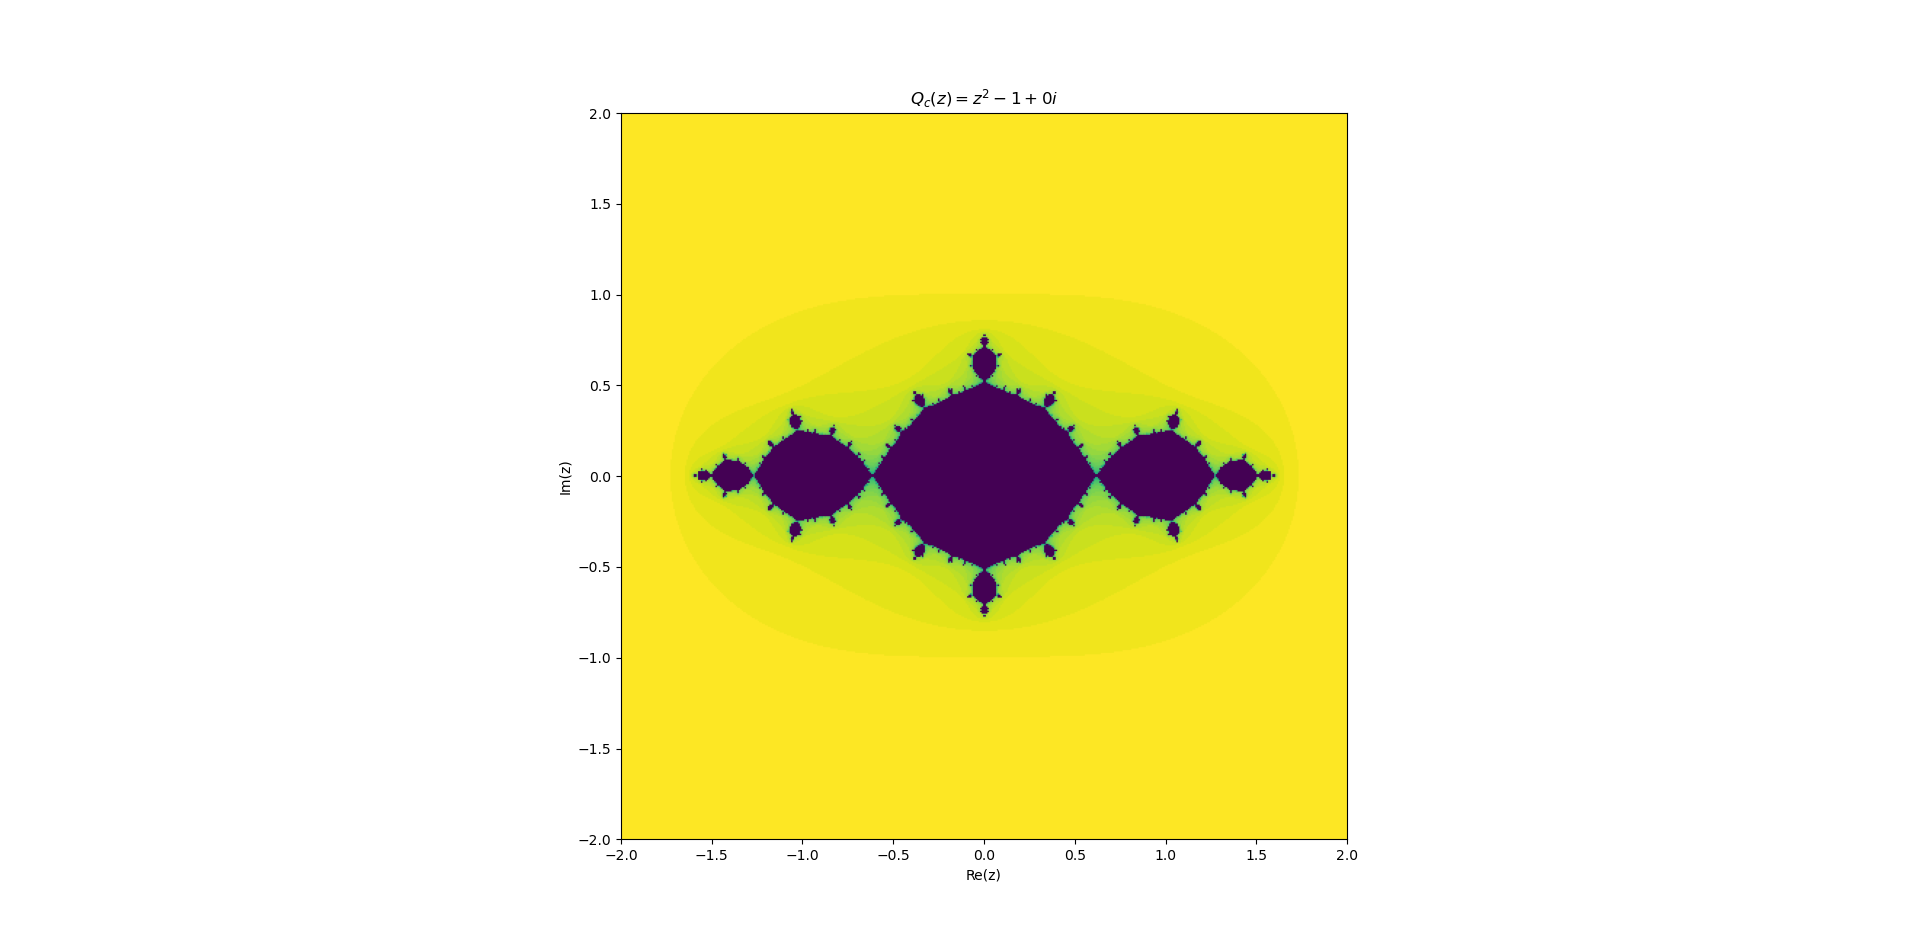
\includegraphics[width=3in]{./Figure_1.png}
\end{figure}
\vspace{-.2in}

\begin{abstract}
	In this research project we study the Julia sets of the complex quadratic
	function $Q^k_c\colon z \mapsto z^2 + c$, for complex $c$. Julia sets
	represent the chaotic dynamics of complex functions and are visualized by
	repeatedly applying the complex function to `seed' points in the complex plane.
	In this project we understand the theoretical reasoning of the
	escape criteria $Q^k_c(z) > \operatorname{max}\{|c|, 2\}$ to  produce images
	of the filled Julia sets using code written in Python using NumPy
	and Matplotlib for visualization, as well as through GPU shaders.
	We observe that the connectedness property
	changes abruptly as we take $c$ increasingly further from the origin.
	\begin{figure}[htb!]
		\centering
	\end{figure}
\end{abstract}

\end{document}
